\documentclass[12pt,landscape]{article}

%\usepackage{lmodern}
\usepackage{amssymb,amsmath}
\usepackage{bm}
\usepackage{graphicx}
\usepackage{microtype}
\usepackage{hyperref}
\pagestyle{empty}
\usepackage{titlesec}
\titleformat*{\section}{\LARGE\bfseries}
\titleformat*{\subsection}{\LARGE\bfseries}
\titleformat*{\subsubsection}{\LARGE\bfseries}
\setlength{\parindent}{0pt}
\setlength{\parskip}{1.2ex}
\setlength{\parindent}{0pt}
\setlength{\parskip}{1.2ex}

\setlength{\oddsidemargin}{-16mm}
\setlength{\textwidth}{260mm}
\setlength{\columnsep}{0.5in}
\setlength{\columnseprule}{1pt}
\setlength{\textheight}{202mm}
\setlength{\topmargin}{-32mm}
\setlength{\headsep}{0.25in}

\hypersetup
       {   pdfauthor = { Marco Fasondini },
           pdftitle={ foo },
           colorlinks=TRUE,
           linkcolor=black,
           citecolor=blue,
           urlcolor=blue
       }




\usepackage{upquote}
\usepackage{listings}
\usepackage{xcolor}
\lstset{
    basicstyle=\ttfamily\footnotesize,
    upquote=true,
    breaklines=true,
    breakindent=0pt,
    keepspaces=true,
    showspaces=false,
    columns=fullflexible,
    showtabs=false,
    showstringspaces=false,
    escapeinside={(*@}{@*)},
    extendedchars=true,
}
\newcommand{\HLJLt}[1]{#1}
\newcommand{\HLJLw}[1]{#1}
\newcommand{\HLJLe}[1]{#1}
\newcommand{\HLJLeB}[1]{#1}
\newcommand{\HLJLo}[1]{#1}
\newcommand{\HLJLk}[1]{\textcolor[RGB]{148,91,176}{\textbf{#1}}}
\newcommand{\HLJLkc}[1]{\textcolor[RGB]{59,151,46}{\textit{#1}}}
\newcommand{\HLJLkd}[1]{\textcolor[RGB]{214,102,97}{\textit{#1}}}
\newcommand{\HLJLkn}[1]{\textcolor[RGB]{148,91,176}{\textbf{#1}}}
\newcommand{\HLJLkp}[1]{\textcolor[RGB]{148,91,176}{\textbf{#1}}}
\newcommand{\HLJLkr}[1]{\textcolor[RGB]{148,91,176}{\textbf{#1}}}
\newcommand{\HLJLkt}[1]{\textcolor[RGB]{148,91,176}{\textbf{#1}}}
\newcommand{\HLJLn}[1]{#1}
\newcommand{\HLJLna}[1]{#1}
\newcommand{\HLJLnb}[1]{#1}
\newcommand{\HLJLnbp}[1]{#1}
\newcommand{\HLJLnc}[1]{#1}
\newcommand{\HLJLncB}[1]{#1}
\newcommand{\HLJLnd}[1]{\textcolor[RGB]{214,102,97}{#1}}
\newcommand{\HLJLne}[1]{#1}
\newcommand{\HLJLneB}[1]{#1}
\newcommand{\HLJLnf}[1]{\textcolor[RGB]{66,102,213}{#1}}
\newcommand{\HLJLnfm}[1]{\textcolor[RGB]{66,102,213}{#1}}
\newcommand{\HLJLnp}[1]{#1}
\newcommand{\HLJLnl}[1]{#1}
\newcommand{\HLJLnn}[1]{#1}
\newcommand{\HLJLno}[1]{#1}
\newcommand{\HLJLnt}[1]{#1}
\newcommand{\HLJLnv}[1]{#1}
\newcommand{\HLJLnvc}[1]{#1}
\newcommand{\HLJLnvg}[1]{#1}
\newcommand{\HLJLnvi}[1]{#1}
\newcommand{\HLJLnvm}[1]{#1}
\newcommand{\HLJLl}[1]{#1}
\newcommand{\HLJLld}[1]{\textcolor[RGB]{148,91,176}{\textit{#1}}}
\newcommand{\HLJLs}[1]{\textcolor[RGB]{201,61,57}{#1}}
\newcommand{\HLJLsa}[1]{\textcolor[RGB]{201,61,57}{#1}}
\newcommand{\HLJLsb}[1]{\textcolor[RGB]{201,61,57}{#1}}
\newcommand{\HLJLsc}[1]{\textcolor[RGB]{201,61,57}{#1}}
\newcommand{\HLJLsd}[1]{\textcolor[RGB]{201,61,57}{#1}}
\newcommand{\HLJLsdB}[1]{\textcolor[RGB]{201,61,57}{#1}}
\newcommand{\HLJLsdC}[1]{\textcolor[RGB]{201,61,57}{#1}}
\newcommand{\HLJLse}[1]{\textcolor[RGB]{59,151,46}{#1}}
\newcommand{\HLJLsh}[1]{\textcolor[RGB]{201,61,57}{#1}}
\newcommand{\HLJLsi}[1]{#1}
\newcommand{\HLJLso}[1]{\textcolor[RGB]{201,61,57}{#1}}
\newcommand{\HLJLsr}[1]{\textcolor[RGB]{201,61,57}{#1}}
\newcommand{\HLJLss}[1]{\textcolor[RGB]{201,61,57}{#1}}
\newcommand{\HLJLssB}[1]{\textcolor[RGB]{201,61,57}{#1}}
\newcommand{\HLJLnB}[1]{\textcolor[RGB]{59,151,46}{#1}}
\newcommand{\HLJLnbB}[1]{\textcolor[RGB]{59,151,46}{#1}}
\newcommand{\HLJLnfB}[1]{\textcolor[RGB]{59,151,46}{#1}}
\newcommand{\HLJLnh}[1]{\textcolor[RGB]{59,151,46}{#1}}
\newcommand{\HLJLni}[1]{\textcolor[RGB]{59,151,46}{#1}}
\newcommand{\HLJLnil}[1]{\textcolor[RGB]{59,151,46}{#1}}
\newcommand{\HLJLnoB}[1]{\textcolor[RGB]{59,151,46}{#1}}
\newcommand{\HLJLoB}[1]{\textcolor[RGB]{102,102,102}{\textbf{#1}}}
\newcommand{\HLJLow}[1]{\textcolor[RGB]{102,102,102}{\textbf{#1}}}
\newcommand{\HLJLp}[1]{#1}
\newcommand{\HLJLc}[1]{\textcolor[RGB]{153,153,119}{\textit{#1}}}
\newcommand{\HLJLch}[1]{\textcolor[RGB]{153,153,119}{\textit{#1}}}
\newcommand{\HLJLcm}[1]{\textcolor[RGB]{153,153,119}{\textit{#1}}}
\newcommand{\HLJLcp}[1]{\textcolor[RGB]{153,153,119}{\textit{#1}}}
\newcommand{\HLJLcpB}[1]{\textcolor[RGB]{153,153,119}{\textit{#1}}}
\newcommand{\HLJLcs}[1]{\textcolor[RGB]{153,153,119}{\textit{#1}}}
\newcommand{\HLJLcsB}[1]{\textcolor[RGB]{153,153,119}{\textit{#1}}}
\newcommand{\HLJLg}[1]{#1}
\newcommand{\HLJLgd}[1]{#1}
\newcommand{\HLJLge}[1]{#1}
\newcommand{\HLJLgeB}[1]{#1}
\newcommand{\HLJLgh}[1]{#1}
\newcommand{\HLJLgi}[1]{#1}
\newcommand{\HLJLgo}[1]{#1}
\newcommand{\HLJLgp}[1]{#1}
\newcommand{\HLJLgs}[1]{#1}
\newcommand{\HLJLgsB}[1]{#1}
\newcommand{\HLJLgt}[1]{#1}



\def\qqand{\qquad\hbox{and}\qquad}
\def\qqfor{\qquad\hbox{for}\qquad}
\def\qqas{\qquad\hbox{as}\qquad}
\def\half{ {1 \over 2} }
\def\D{ {\rm d} }
\def\I{ {\rm i} }
\def\E{ {\rm e} }
\def\C{ {\mathbb C} }
\def\R{ {\mathbb R} }
\def\H{ {\mathbb H} }
\def\Z{ {\mathbb Z} }
\def\CC{ {\cal C} }
\def\FF{ {\cal F} }
\def\HH{ {\cal H} }
\def\LL{ {\cal L} }
\def\vc#1{ {\mathbf #1} }
\def\bbC{ {\mathbb C} }



\def\fR{ f_{\rm R} }
\def\fL{ f_{\rm L} }

\def\qqqquad{\qquad\qquad}
\def\qqwhere{\qquad\hbox{where}\qquad}
\def\Res_#1{\underset{#1}{\rm Res}\,}
\def\sech{ {\rm sech}\, }
\def\acos{ {\rm acos}\, }
\def\asin{ {\rm asin}\, }
\def\atan{ {\rm atan}\, }
\def\Ei{ {\rm Ei}\, }
\def\upepsilon{\varepsilon}


\def\Xint#1{ \mathchoice
   {\XXint\displaystyle\textstyle{#1} }%
   {\XXint\textstyle\scriptstyle{#1} }%
   {\XXint\scriptstyle\scriptscriptstyle{#1} }%
   {\XXint\scriptscriptstyle\scriptscriptstyle{#1} }%
   \!\int}
\def\XXint#1#2#3{ {\setbox0=\hbox{$#1{#2#3}{\int}$}
     \vcenter{\hbox{$#2#3$}}\kern-.5\wd0} }
\def\ddashint{\Xint=}
\def\dashint{\Xint-}
% \def\dashint
\def\infdashint{\dashint_{-\infty}^\infty}




\def\addtab#1={#1\;&=}
\def\ccr{\\\addtab}
\def\ip<#1>{\left\langle{#1}\right\rangle}
\def\dx{\D x}
\def\dt{\D t}
\def\dz{\D z}
\def\ds{\D s}

\def\rR{ {\rm R} }
\def\rL{ {\rm L} }

\def\norm#1{\left\| #1 \right\|}

\def\pr(#1){\left({#1}\right)}
\def\br[#1]{\left[{#1}\right]}

\def\abs#1{\left|{#1}\right|}
\def\fpr(#1){\!\pr({#1})}

\def\sopmatrix#1{ \begin{pmatrix}#1\end{pmatrix} }

\def\endash{–}
\def\emdash{—}
\def\mdblksquare{\blacksquare}
\def\lgblksquare{\blacksquare}
\def\scre{\E}
\def\mapengine#1,#2.{\mapfunction{#1}\ifx\void#2\else\mapengine #2.\fi }

\def\map[#1]{\mapengine #1,\void.}

\def\mapenginesep_#1#2,#3.{\mapfunction{#2}\ifx\void#3\else#1\mapengine #3.\fi }

\def\mapsep_#1[#2]{\mapenginesep_{#1}#2,\void.}


\def\vcbr[#1]{\pr(#1)}


\def\bvect[#1,#2]{
{
\def\dots{\cdots}
\def\mapfunction##1{\ | \  ##1}
	\sopmatrix{
		 \,#1\map[#2]\,
	}
}
}



\def\vect[#1]{
{\def\dots{\ldots}
	\vcbr[{#1}]
} }

\def\vectt[#1]{
{\def\dots{\ldots}
	\vect[{#1}]^{\top}
} }

\def\Vectt[#1]{
{
\def\mapfunction##1{##1 \cr}
\def\dots{\vdots}
	\begin{pmatrix}
		\map[#1]
	\end{pmatrix}
} }

\def\addtab#1={#1\;&=}
\def\ccr{\\\addtab}

\def\questionequals{= \!\!\!\!\!\!{\scriptstyle ? \atop }\,\,\,}

\def\cent#1{\begin{center}#1\end{center} }

\lstset{
    basicstyle=\ttfamily,
	}

\begin{document}
{\LARGE
\sf
\textbf{Applied Complex Analysis (2021)}

\section{Lecture 26: The Wiener-Hopf method}
The Wiener\ensuremath{\endash}Hopf method is an approach for solving integral equations of the form

\[
\lambda u(x) + \int_0^\infty K(x-t)u(t) \dt = f(x)\qqfor 0 \leq x < \infty.
\]
Here $f$ and $K$ are given functions, $\lambda$ is a given constant, and we want to find $u$. The approach similarly extends to integro-differential equations of the form

\[
c_1 u''(x) + c_2 u'(x) + \lambda u(x) + \int_0^\infty K(x-t)u(t) \dt = f(x)\qqfor 0 \leq x < \infty.
\]
Here $c_1, c_2, \lambda$ are given constants and again we want to find $u$.

In this course, we will only consider $K(x) = \E^{-\gamma |x|}$, though the methodology translates to other choices of $K$.

\section{Integral equations on the real line}
Before discussing problems on the half line, we consider problems on the whole line:

\[
\lambda u(x) + \int_{-\infty}^\infty K(x-t)u(t) \dt = f(x)\qqfor -\infty < x < \infty.
\]
Outline:

Recall the Fourier transform of a function (using $s$ so I don't get confused with $K$):

\[
    {\hat{K}}(s) = {\cal F} K (s) =  \int_{-\infty}^\infty K(t) \E^{-\I s t} \dt
\]
so that

\[
K(x) = {\cal F}^{-1} \hat K(x) =  {1 \over 2\pi}\int_{-\infty}^\infty \hat K(s) \E^{ \I s x} \D s
\]
What effect does translating a function have on it's Fourier transform?

\[
\int_{-\infty}^\infty K(t+x_0) \E^{-\I s t} \dt = \int_{-\infty}^\infty K(\tau) \E^{-\I s (\tau - x_0)} \dt = \E^{\I s x_0} \hat K(s)
\]
We are interested in the  Fourier transform of the \emph{convolution} term

\[
\int_{-\infty}^\infty K(x-t)u(t) \dt
\]
But we have

\[
\int_{-\infty}^\infty \E^{-\I s x} \int_{-\infty}^\infty K(x-t)u(t) \dt \dx = \int_{-\infty}^\infty \int_{-\infty}^\infty \E^{-\I s x} K(x-t)\dx u(t) \dt =
\int_{-\infty}^\infty \E^{-\I s t} \hat K(s) u(t) \dt = \hat K(s) \hat u(s)
\]
That is, convolution becomes multiplication. Thus our integral equation in Fourier space becomes:

\[
(\lambda + \hat K(s)) \hat u(s) = \hat f(s) \qqfor -\infty < s < \infty
\]
Or in other words,

\[
u(x) = {\cal F}^{-1} \left[{\hat f \over \lambda + \hat K }\right](x)
\]
\subsubsection{Example:}
Consider the kernel $K(x) = \E^{-\gamma |x|}$. Then we have


\begin{align*}
\hat K(s) &= \int_{-\infty}^\infty K(t) \E^{-\I s t} \dt = \int_{-\infty}^0 \E^{( \gamma - \I s ) t} \dt  + \int_0^\infty \E^{(-\gamma - \I s ) t} = {1 \over  \gamma - \I s} - {1 \over -\gamma - \I s } \\
&= {2\gamma \over \gamma^2 + s^2}
\end{align*}

\begin{lstlisting}
(*@\HLJLk{using}@*) (*@\HLJLn{Plots}@*)(*@\HLJLp{,}@*) (*@\HLJLn{ComplexPhasePortrait}@*)(*@\HLJLp{,}@*) (*@\HLJLn{ApproxFun}@*)(*@\HLJLp{,}@*) (*@\HLJLn{SingularIntegralEquations}@*)(*@\HLJLp{,}@*) (*@\HLJLn{OscillatoryIntegrals}@*)
(*@\HLJLk{import}@*) (*@\HLJLn{ApproxFun}@*)(*@\HLJLoB{:}@*) (*@\HLJLn{UnionDomain}@*)

(*@\HLJLn{\ensuremath{\gamma}}@*) (*@\HLJLoB{=}@*) (*@\HLJLnfB{2.0}@*)
(*@\HLJLn{\ensuremath{\Gamma}}@*) (*@\HLJLoB{=}@*) (*@\HLJLn{ApproxFun}@*)(*@\HLJLoB{.}@*)(*@\HLJLnf{UnionDomain}@*)(*@\HLJLp{((}@*)(*@\HLJLoB{-}@*)(*@\HLJLn{Inf}@*) (*@\HLJLoB{..}@*) (*@\HLJLni{0}@*)(*@\HLJLp{)}@*) (*@\HLJLp{,}@*) (*@\HLJLp{(}@*)(*@\HLJLni{0}@*) (*@\HLJLoB{..}@*) (*@\HLJLn{Inf}@*)(*@\HLJLp{))}@*) (*@\HLJLcs{{\#}}@*) (*@\HLJLcs{Line}@*) (*@\HLJLcs{split}@*) (*@\HLJLcs{in}@*) (*@\HLJLcs{two}@*)
(*@\HLJLn{K}@*) (*@\HLJLoB{=}@*) (*@\HLJLnf{Fun}@*)(*@\HLJLp{(}@*)(*@\HLJLn{x}@*) (*@\HLJLoB{->}@*) (*@\HLJLnf{exp}@*)(*@\HLJLp{(}@*)(*@\HLJLoB{-}@*)(*@\HLJLn{\ensuremath{\gamma}}@*)(*@\HLJLoB{*}@*)(*@\HLJLnf{abs}@*)(*@\HLJLp{(}@*)(*@\HLJLn{x}@*)(*@\HLJLp{)),}@*) (*@\HLJLn{\ensuremath{\Gamma}}@*)(*@\HLJLp{)}@*)
(*@\HLJLn{Kh}@*) (*@\HLJLoB{=}@*) (*@\HLJLn{s}@*) (*@\HLJLoB{->}@*) (*@\HLJLnf{fourier}@*)(*@\HLJLp{(}@*)(*@\HLJLn{K}@*)(*@\HLJLp{,}@*) (*@\HLJLoB{-}@*)(*@\HLJLn{s}@*)(*@\HLJLp{)}@*) (*@\HLJLcs{{\#}}@*) (*@\HLJLcs{magic}@*) (*@\HLJLcs{routine}@*) (*@\HLJLcs{for}@*) (*@\HLJLcs{Fourier}@*) (*@\HLJLcs{transforms}@*)
(*@\HLJLnf{Kh}@*)(*@\HLJLp{(}@*)(*@\HLJLnfB{2.0}@*)(*@\HLJLp{)}@*) (*@\HLJLp{,}@*) (*@\HLJLni{2}@*)(*@\HLJLn{\ensuremath{\gamma}}@*)(*@\HLJLoB{/}@*)(*@\HLJLp{(}@*)(*@\HLJLn{\ensuremath{\gamma}}@*)(*@\HLJLoB{{\textasciicircum}}@*)(*@\HLJLni{2}@*)(*@\HLJLoB{+}@*)(*@\HLJLnfB{2.0}@*)(*@\HLJLoB{{\textasciicircum}}@*)(*@\HLJLni{2}@*)(*@\HLJLp{)}@*)
\end{lstlisting}

\begin{lstlisting}
(0.4999999999996446 + 0.0im, 0.5)
\end{lstlisting}


Consider a simple RHS like

\[
f(x) = {1 \over x^2 + a^2}
\]
Because of the decay, we can use Residue calculus to determine, for $s < 0$ deforming to the upper half plane,

\[
\hat f(s) = \int_{-\infty}^\infty {\E^{-\I s t} \over t^2 + a^2}\dt = 2 \pi \I \Res_{z = a \I}{\E^{-\I s z} \over z^2 + a^2} = \pi  {\E^{s a} \over a}
\]
and for $s > 0$ deforming to the lower half plane

\[
\hat f(s) =-2 \pi \I \Res_{z =- a \I}{\E^{-\I s z} \over z^2 + a^2} = \pi {\E^{-s a} \over  a}
\]
and for $s = 0$ the results match:

\[
\hat f(0) = {\pi  \over  a}
\]
\textbf{Remark} The Fourier transform of smooth functions that exponentially decay are smooth functions that exponentially decay. When we only have algebraic decay, that indicates that the Fourier transform is smooth apart from at $0$.


\begin{lstlisting}
(*@\HLJLn{a}@*) (*@\HLJLoB{=}@*) (*@\HLJLnfB{2.0}@*)
(*@\HLJLn{f}@*) (*@\HLJLoB{=}@*) (*@\HLJLnf{Fun}@*)(*@\HLJLp{(}@*)(*@\HLJLn{x}@*) (*@\HLJLoB{->}@*) (*@\HLJLni{1}@*)(*@\HLJLoB{/}@*)(*@\HLJLp{(}@*)(*@\HLJLn{x}@*)(*@\HLJLoB{{\textasciicircum}}@*)(*@\HLJLni{2}@*) (*@\HLJLoB{+}@*) (*@\HLJLn{a}@*)(*@\HLJLoB{{\textasciicircum}}@*)(*@\HLJLni{2}@*)(*@\HLJLp{),}@*) (*@\HLJLn{\ensuremath{\Gamma}}@*)(*@\HLJLp{)}@*)
(*@\HLJLn{fh}@*) (*@\HLJLoB{=}@*) (*@\HLJLn{s}@*) (*@\HLJLoB{->}@*) (*@\HLJLnf{fourier}@*)(*@\HLJLp{(}@*)(*@\HLJLn{f}@*)(*@\HLJLp{,}@*) (*@\HLJLoB{-}@*)(*@\HLJLn{s}@*)(*@\HLJLp{)}@*)
(*@\HLJLnf{fh}@*)(*@\HLJLp{(}@*)(*@\HLJLni{0}@*)(*@\HLJLp{)}@*) (*@\HLJLoB{-}@*) (*@\HLJLn{\ensuremath{\pi}}@*)(*@\HLJLoB{/}@*)(*@\HLJLn{a}@*)

(*@\HLJLnf{fh}@*)(*@\HLJLp{(}@*)(*@\HLJLnfB{2.0}@*)(*@\HLJLp{)}@*) (*@\HLJLoB{-}@*) (*@\HLJLp{(}@*)(*@\HLJLn{\ensuremath{\pi}}@*)(*@\HLJLoB{*}@*)(*@\HLJLnf{exp}@*)(*@\HLJLp{(}@*)(*@\HLJLoB{-}@*)(*@\HLJLnfB{2.0}@*)(*@\HLJLoB{*}@*)(*@\HLJLn{a}@*)(*@\HLJLp{)}@*)(*@\HLJLoB{/}@*)(*@\HLJLn{a}@*)(*@\HLJLp{),}@*) (*@\HLJLnf{fh}@*)(*@\HLJLp{(}@*)(*@\HLJLoB{-}@*)(*@\HLJLnfB{2.0}@*)(*@\HLJLp{)}@*) (*@\HLJLoB{-}@*) (*@\HLJLp{(}@*)(*@\HLJLn{\ensuremath{\pi}}@*)(*@\HLJLoB{*}@*)(*@\HLJLnf{exp}@*)(*@\HLJLp{(}@*)(*@\HLJLoB{-}@*)(*@\HLJLnfB{2.0}@*)(*@\HLJLoB{*}@*)(*@\HLJLn{a}@*)(*@\HLJLp{)}@*)(*@\HLJLoB{/}@*)(*@\HLJLn{a}@*)(*@\HLJLp{)}@*)
\end{lstlisting}

\begin{lstlisting}
(1.214306433183765e-16 - 5.551115123125783e-17im, 1.214306433183765e-16 + 5
.551115123125783e-17im)
\end{lstlisting}


So we can now solve the integral equation

\[
\lambda u(x) + \int_{-\infty}^\infty K(x-t)u(t) \dt = f(x)\qqfor -\infty < x < \infty.
\]
by converting to Fourier space

\[
(\lambda + \hat K(s)) \hat u(s)  = \hat f(s)\qqfor -\infty < x < \infty.
\]
to get

\[
\hat u(s) = {\pi \over a} { \E^{-a |s|} (\gamma^2+s^2) \over \lambda (\gamma^2+s^2) + 2\gamma}
\]
Therefore, $u(x)$ is the inverse Fourier transform of this. We calculate it numerically first:


\begin{lstlisting}
(*@\HLJLn{\ensuremath{\lambda}}@*) (*@\HLJLoB{=}@*) (*@\HLJLnfB{1.0}@*)
(*@\HLJLn{uh}@*) (*@\HLJLoB{=}@*) (*@\HLJLn{\ensuremath{\pi}}@*)(*@\HLJLoB{/}@*)(*@\HLJLn{a}@*)(*@\HLJLoB{*}@*)(*@\HLJLnf{Fun}@*)(*@\HLJLp{(}@*)(*@\HLJLn{s}@*) (*@\HLJLoB{->}@*) (*@\HLJLnf{exp}@*)(*@\HLJLp{(}@*)(*@\HLJLoB{-}@*)(*@\HLJLn{a}@*)(*@\HLJLoB{*}@*)(*@\HLJLnf{abs}@*)(*@\HLJLp{(}@*)(*@\HLJLn{s}@*)(*@\HLJLp{))}@*)(*@\HLJLoB{*}@*)(*@\HLJLp{(}@*)(*@\HLJLn{\ensuremath{\gamma}}@*)(*@\HLJLoB{{\textasciicircum}}@*)(*@\HLJLni{2}@*) (*@\HLJLoB{+}@*) (*@\HLJLn{s}@*)(*@\HLJLoB{{\textasciicircum}}@*)(*@\HLJLni{2}@*)(*@\HLJLp{)}@*)(*@\HLJLoB{/}@*)(*@\HLJLp{(}@*)(*@\HLJLn{\ensuremath{\lambda}}@*)(*@\HLJLoB{*}@*)(*@\HLJLp{(}@*)(*@\HLJLn{\ensuremath{\gamma}}@*)(*@\HLJLoB{{\textasciicircum}}@*)(*@\HLJLni{2}@*) (*@\HLJLoB{+}@*) (*@\HLJLn{s}@*)(*@\HLJLoB{{\textasciicircum}}@*)(*@\HLJLni{2}@*)(*@\HLJLp{)}@*) (*@\HLJLoB{+}@*) (*@\HLJLni{2}@*)(*@\HLJLn{\ensuremath{\gamma}}@*)(*@\HLJLp{),}@*) (*@\HLJLn{\ensuremath{\Gamma}}@*)(*@\HLJLp{)}@*)

(*@\HLJLn{u}@*) (*@\HLJLoB{=}@*) (*@\HLJLnf{Fun}@*)(*@\HLJLp{(}@*)(*@\HLJLn{x}@*) (*@\HLJLoB{->}@*) (*@\HLJLnf{fourier}@*)(*@\HLJLp{(}@*)(*@\HLJLn{uh}@*)(*@\HLJLp{,}@*) (*@\HLJLn{x}@*)(*@\HLJLp{),}@*) (*@\HLJLn{\ensuremath{\Gamma}}@*)(*@\HLJLp{)}@*)(*@\HLJLoB{/}@*)(*@\HLJLp{(}@*)(*@\HLJLni{2}@*)(*@\HLJLn{\ensuremath{\pi}}@*)(*@\HLJLp{)}@*)

(*@\HLJLnf{plot}@*)(*@\HLJLp{(}@*)(*@\HLJLoB{-}@*)(*@\HLJLnfB{10.0}@*)(*@\HLJLoB{:}@*)(*@\HLJLnfB{0.1}@*)(*@\HLJLoB{:}@*)(*@\HLJLnfB{10.0}@*)(*@\HLJLp{,}@*) (*@\HLJLn{u}@*)(*@\HLJLp{)}@*)
\end{lstlisting}

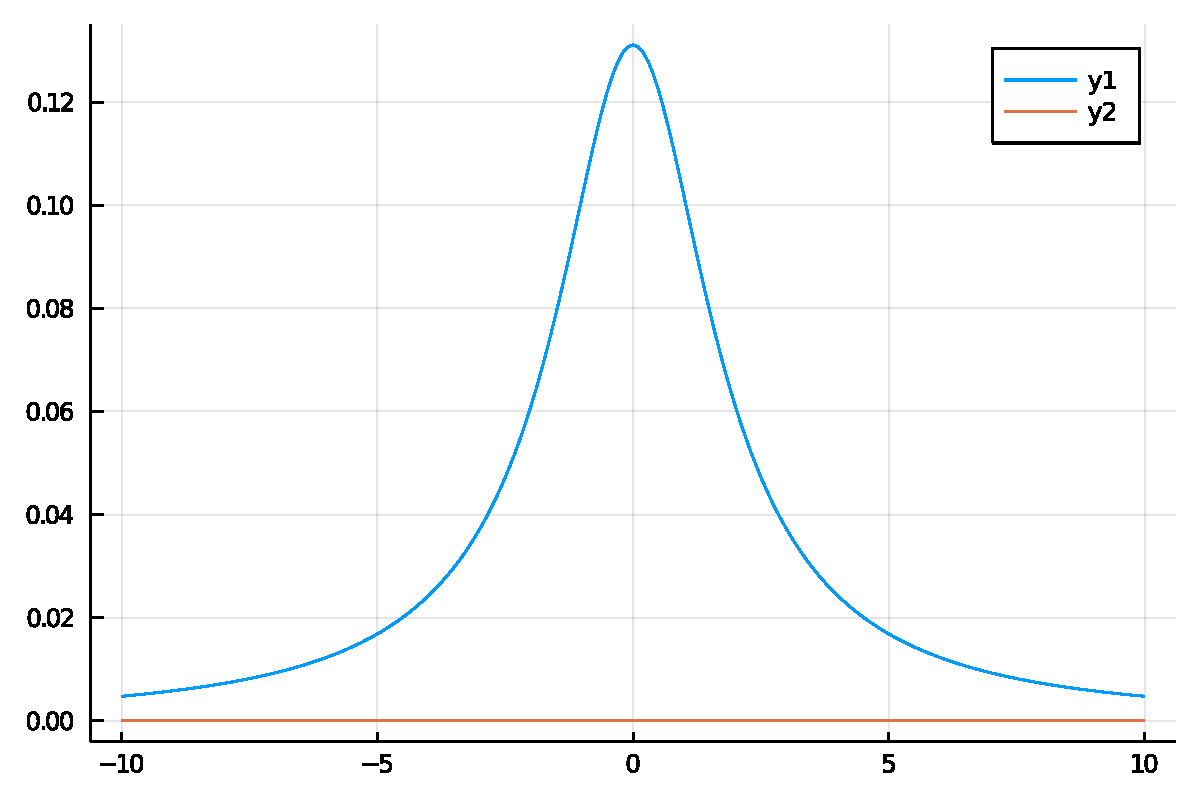
\includegraphics[width=\linewidth]{C:/Users/mfaso/OneDrive/Documents/GitHub/M3M6AppliedComplexAnalysis/output/figures/Lecture26_3_1.pdf}

\begin{lstlisting}
(*@\HLJLn{\ensuremath{\lambda}}@*)(*@\HLJLoB{*}@*)(*@\HLJLnf{u}@*)(*@\HLJLp{(}@*)(*@\HLJLnfB{0.0}@*)(*@\HLJLp{)}@*) (*@\HLJLoB{+}@*)  (*@\HLJLnf{sum}@*)(*@\HLJLp{(}@*)(*@\HLJLn{u}@*)(*@\HLJLoB{*}@*)(*@\HLJLn{K}@*)(*@\HLJLp{),}@*) (*@\HLJLnf{f}@*)(*@\HLJLp{(}@*)(*@\HLJLnfB{0.0}@*)(*@\HLJLp{)}@*)
\end{lstlisting}

\begin{lstlisting}
(0.24999999999993416 + 2.949231154457839e-19im, 0.25)
\end{lstlisting}


\begin{lstlisting}
(*@\HLJLn{x}@*) (*@\HLJLoB{=}@*)(*@\HLJLnfB{2.0}@*)
(*@\HLJLn{\ensuremath{\lambda}}@*)(*@\HLJLoB{*}@*)(*@\HLJLnf{u}@*)(*@\HLJLp{(}@*)(*@\HLJLn{x}@*)(*@\HLJLp{)}@*) (*@\HLJLoB{+}@*)  (*@\HLJLnf{sum}@*)(*@\HLJLp{(}@*)(*@\HLJLnf{Fun}@*)(*@\HLJLp{(}@*)(*@\HLJLn{t}@*) (*@\HLJLoB{->}@*) (*@\HLJLnf{K}@*)(*@\HLJLp{(}@*)(*@\HLJLn{x}@*)(*@\HLJLoB{-}@*)(*@\HLJLn{t}@*)(*@\HLJLp{)}@*)(*@\HLJLoB{*}@*)(*@\HLJLnf{u}@*)(*@\HLJLp{(}@*)(*@\HLJLn{t}@*)(*@\HLJLp{),}@*) (*@\HLJLnf{UnionDomain}@*)(*@\HLJLp{(}@*)(*@\HLJLoB{-}@*)(*@\HLJLn{Inf}@*) (*@\HLJLoB{..}@*) (*@\HLJLn{x}@*)(*@\HLJLp{,}@*) (*@\HLJLn{x}@*) (*@\HLJLoB{..}@*) (*@\HLJLn{Inf}@*)(*@\HLJLp{)))}@*) (*@\HLJLp{,}@*) (*@\HLJLnf{f}@*)(*@\HLJLp{(}@*)(*@\HLJLn{x}@*)(*@\HLJLp{)}@*)
\end{lstlisting}

\begin{lstlisting}
(0.12499999999949421 - 5.459951382663637e-16im, 0.12500000000000003)
\end{lstlisting}


Working out the analytic formula for this example takes a lot more work and involves other special functions, and is outside the scope of the course.

\section{Integral equations on the half-line and Riemann\ensuremath{\endash}Hilbert problems}
Taking Fourier transforms, we get functions analytic above or below the real axis, giving us a Riemann\ensuremath{\endash}Hilbert problem of finding $\Phi(z)$ analytic off $(-\infty,\infty)$ such that

\[
\Phi_+(s) - g(s)\Phi_-(s) = h(s) \qqand \Phi(\infty) = C
\]
where $\Phi_\pm(s) = \lim_{\epsilon \rightarrow 0} \Phi(s \pm \I \epsilon)$ are the limits from above and below.  Here $g$ and $h$ are given, and $g(\pm \infty) = 1$.

Recall the notation

\[
f_{\rm R}(x) = \begin{cases}f(t) & t \geq 0 \\ 0 & \hbox{otherwise} \end{cases}
\]
and

\[
f_{\rm L}(x) = \begin{cases}f(t) & t < 0 \\ 0 & \hbox{otherwise} \end{cases}
\]
Using this, we can rewrite the integral equation on the half line

\[
\lambda u(x) + \int_{0}^\infty K(x-t)u(t) \dt = f(x)\qqfor 0 < x < \infty.
\]
as an integral equation on the whole line:

\[
\lambda u_{\rm R}(x) + \int_{-\infty}^\infty K(x-t)u_{\rm R}(t) \dt = f_{\rm R}(x) + p_{\rm L}(x)\qqfor -\infty < x < \infty.
\]
where

\[
p(x) = \int_{-\infty}^\infty K(x-t)u_{\rm R}(t) \dt
\]
Taking Fourier transforms, this becomes:

\[
(\lambda + \widehat K(s)) \widehat{u_{\rm R}}(s) = \widehat{f_{\rm R}}(s) + \widehat{p_{\rm L}}(s)
\]
As discussed last lecture, assuming $u$ is "nice" we are guaranteed that $\widehat{ u_{\rm R}}(s)$ is analytic in the lower half-plane and $\widehat{ p_{\rm L}}(s)$ is analytic in the upper-half plane. Thus introduce the sectionally analytic function:

\[
\Phi(z) = \begin{cases}  \widehat{p_{\rm L}}(z) & \Im z > 0 \\
                            \widehat{u_{\rm R}}(z) & \Im z < 0
                            \end{cases}
\]
Then our integral transformed integral equation becomes:

\[
\underbrace{\Phi_+(s)}_{\widehat{p_{\rm L}}(s)} - \underbrace{g(s)}_{\lambda + \widehat K(s)} \underbrace{\Phi_-(s)}_{\widehat{u_{\rm R}}(s)} = \underbrace{h(s)}_{-\widehat{f_{\rm R}}(s) } \qqand \Phi(\infty) = 0
\]
Here there is one unknown $\Phi(z)$, and we claim that in certain conditions this has one\ensuremath{\emdash}and only\ensuremath{\emdash}one solution. Thus we wish to:

\begin{itemize}
\item[1. ] Find $\Phi(z)$


\item[2. ] Recover $u(x)$ via the inverse Fourier transform ${\cal F}^{-1} \Phi_-$

\end{itemize}
\section{The Wiener\ensuremath{\endash}Hopf method: an example}
We can now employ the Wiener\ensuremath{\endash}Hopf method to solve

\[
\lambda u(x) + \int_{0}^\infty K(x-t)u(t) \dt = f(x)\qqfor 0 < x < \infty.
\]
The Wiener\ensuremath{\endash}Hopf method consists of the following steps:

\begin{itemize}
\item[1. ] Calculate Fourier transforms $\widehat K(s)$ and $\widehat{f_{\rm R}}(s)$ to reduce to RH problem

\end{itemize}
\[
\Phi_+(s) -g(s) \Phi_-(s) = h(s)
\]
with $\lim \Phi(z) = 0$

\begin{itemize}
\item[2. ] Find homogenous solution $\kappa_+(s) = g(s) \kappa_-(s)$ with $\lim \kappa(z) = 1$


\item[3. ] Solve Cauchy transform problem $Y_+(s) - Y_-(s) = {h(s) \over \kappa_+(s)}$


\item[4. ] Find $u(x)$ by inverting Fourier transform $\widehat{u_{\rm R}}(s) = \Phi_-(s) = \kappa_-(s) Y_-(s)$

\end{itemize}
We will demonstrate these four steps using the example $K(x) = \E^{-|x|}$ and $f(x) = \E^{-x}$, with $\lambda = 1$.

\subsection{Step 1: Calculate Fourier transforms}
We have

\[
\widehat{K}(s) = \int_{-\infty}^0 \E^{t}\E^{-\I s t} \dt + \int_0^\infty \E^{-t} \E^{-\I s t} \dt =
 {1 \over 1-\I s} - {1 \over -1-\I s} = {2 \over 1+s^2}
\]
Because we have exponential decay at $\pm \infty$, $\widehat{K}$ is analytic in a strip. Furthermore,

\[
\widehat{f_{\rm R}}(s) = \int_0^\infty \E^{-t} \E^{-\I t s} \dt = -{1 \over -1-\I s} = {\I \over \I-s}
\]
As predicted, $\widehat{\fR}(s)$ is analytic in the lower half-plane.

We thus have the RH problem:

\[
\underbrace{\Phi_+(s)}_{\widehat{p_{\rm L}}(s)} - \underbrace{g(s)}_{1 + \widehat K(s)}
\underbrace{\Phi_-(s)}_{\widehat{u_{\rm R}}(s)} = \underbrace{h(s)}_{-\widehat{\fR}(s)} \qqand \lim\Phi(z) = 0
\]
where

\[
p(x) = \int_{-\infty}^\infty K(x-t)u_{\rm R}(t) \dt
\]
is unknown, or in our case

\[
\Phi_+(s) - {3 + s^2 \over 1 + s^2} \Phi_-(s) = {\I \over s - \I} \qqand \lim\Phi(z) = 0
\]
Here we confirm our calculations are correct for the Fourier transforms:


\begin{lstlisting}
(*@\HLJLn{t}@*) (*@\HLJLoB{=}@*) (*@\HLJLnf{Fun}@*)(*@\HLJLp{(}@*)(*@\HLJLnfB{0.0}@*) (*@\HLJLoB{..}@*) (*@\HLJLni{40}@*)(*@\HLJLp{)}@*)
(*@\HLJLn{f}@*) (*@\HLJLoB{=}@*) (*@\HLJLnf{exp}@*)(*@\HLJLp{(}@*)(*@\HLJLoB{-}@*)(*@\HLJLn{t}@*)(*@\HLJLp{)}@*)
(*@\HLJLnf{fourier}@*)(*@\HLJLp{(}@*)(*@\HLJLn{f}@*)(*@\HLJLp{,}@*) (*@\HLJLoB{-}@*)(*@\HLJLnfB{2.0}@*)(*@\HLJLp{),}@*) (*@\HLJLn{im}@*)(*@\HLJLoB{/}@*)(*@\HLJLp{(}@*)(*@\HLJLn{im}@*)(*@\HLJLoB{-}@*)(*@\HLJLnfB{2.0}@*)(*@\HLJLp{)}@*)

(*@\HLJLni{1}@*)(*@\HLJLoB{-}@*)(*@\HLJLp{(}@*)(*@\HLJLnf{fourier}@*)(*@\HLJLp{(}@*)(*@\HLJLoB{-}@*)(*@\HLJLnf{exp}@*)(*@\HLJLp{(}@*)(*@\HLJLoB{-}@*)(*@\HLJLn{t}@*)(*@\HLJLp{),}@*) (*@\HLJLoB{-}@*)(*@\HLJLnfB{2.0}@*)(*@\HLJLp{)}@*) (*@\HLJLoB{+}@*) (*@\HLJLnf{fourier}@*)(*@\HLJLp{(}@*)(*@\HLJLoB{-}@*)(*@\HLJLnf{exp}@*)(*@\HLJLp{(}@*)(*@\HLJLnf{Fun}@*)(*@\HLJLp{(}@*)(*@\HLJLoB{-}@*)(*@\HLJLni{40}@*) (*@\HLJLoB{..}@*) (*@\HLJLni{0}@*)(*@\HLJLp{)),}@*) (*@\HLJLoB{-}@*)(*@\HLJLnfB{2.0}@*)(*@\HLJLp{)),}@*) (*@\HLJLp{(}@*)(*@\HLJLnfB{2.0}@*)(*@\HLJLoB{{\textasciicircum}}@*)(*@\HLJLni{2}@*) (*@\HLJLoB{+}@*) (*@\HLJLni{3}@*)(*@\HLJLp{)}@*)(*@\HLJLoB{/}@*)(*@\HLJLp{(}@*)(*@\HLJLnfB{2.0}@*)(*@\HLJLoB{{\textasciicircum}}@*)(*@\HLJLni{2}@*)(*@\HLJLoB{+}@*)(*@\HLJLni{1}@*)(*@\HLJLp{)}@*)
\end{lstlisting}

\begin{lstlisting}
(1.4 - 4.440892098500626e-16im, 1.4)
\end{lstlisting}


\subsection{Step 2: Find homogeneous solution}
Last lecture we employed the "guess and check" kernel factorization method to find

\[
g(s) = {3 + s^2 \over 1 + s^2} = \underbrace{s + \I \sqrt{3} \over s + \I}_{\kappa_+(s)}
\underbrace{s - \I \sqrt{3} \over s-\I }_{\kappa_-(s)^{-1}}
\]
That is, we have the solution

\[
\kappa(z) = \begin{cases} {z + \I \sqrt{3} \over z + \I}  & \Im z > 0 \\
                            {z - \I  \over z - \I \sqrt{3}} & \Im z < 0
                            \end{cases}
\]
Always verify this solution satisfies the right conditions:

\begin{itemize}
\item[1. ] The function $\kappa(z)$ is analytic off $\R$, since the pole of ${z + \I \sqrt{3} \over z + \I}$ is in the lower-half plane and the pole of \$\{z - {\textbackslash}I  {\textbackslash}over z - {\textbackslash}I {\textbackslash}sqrt\{3\}\} \$ is in the upper-half plane


\item[2. ] \[
\lim \kappa(z) = 1
\]
by L'Hopital's rule or similar.


\item[3. ] It has the right jump:

\end{itemize}
\[
\kappa_+(s) = {s + \I \sqrt{3} \over s + \I} = {3 + s^2 \over 1 + s^2}{s - \I  \over s - \I \sqrt{3}} = g(s)\kappa_-(s)
\]
Here we confirm that we have the right jump:


\begin{lstlisting}
(*@\HLJLn{\ensuremath{\kappa}}@*) (*@\HLJLoB{=}@*) (*@\HLJLn{z}@*) (*@\HLJLoB{->}@*) (*@\HLJLnf{imag}@*)(*@\HLJLp{(}@*)(*@\HLJLn{z}@*)(*@\HLJLp{)}@*) (*@\HLJLoB{>}@*) (*@\HLJLni{0}@*) (*@\HLJLoB{?}@*) (*@\HLJLp{(}@*)(*@\HLJLn{z}@*)(*@\HLJLoB{+}@*)(*@\HLJLn{im}@*)(*@\HLJLoB{*}@*)(*@\HLJLnf{sqrt}@*)(*@\HLJLp{(}@*)(*@\HLJLni{3}@*)(*@\HLJLp{))}@*)(*@\HLJLoB{/}@*)(*@\HLJLp{(}@*)(*@\HLJLn{z}@*)(*@\HLJLoB{+}@*)(*@\HLJLn{im}@*)(*@\HLJLp{)}@*) (*@\HLJLoB{:}@*)
                       (*@\HLJLp{(}@*)(*@\HLJLn{z}@*)(*@\HLJLoB{-}@*)(*@\HLJLn{im}@*)(*@\HLJLp{)}@*)(*@\HLJLoB{/}@*)(*@\HLJLp{(}@*)(*@\HLJLn{z}@*)(*@\HLJLoB{-}@*)(*@\HLJLn{im}@*)(*@\HLJLoB{*}@*)(*@\HLJLnf{sqrt}@*)(*@\HLJLp{(}@*)(*@\HLJLni{3}@*)(*@\HLJLp{))}@*)

(*@\HLJLnf{\ensuremath{\kappa}}@*)(*@\HLJLp{(}@*)(*@\HLJLnfB{0.1}@*)(*@\HLJLoB{+}@*)(*@\HLJLnf{eps}@*)(*@\HLJLp{()}@*)(*@\HLJLn{im}@*)(*@\HLJLp{)}@*) (*@\HLJLp{,}@*) (*@\HLJLnf{\ensuremath{\kappa}}@*)(*@\HLJLp{(}@*)(*@\HLJLnfB{0.1}@*)(*@\HLJLoB{-}@*)(*@\HLJLnf{eps}@*)(*@\HLJLp{()}@*)(*@\HLJLn{im}@*)(*@\HLJLp{)}@*)(*@\HLJLoB{*}@*)(*@\HLJLp{(}@*)(*@\HLJLni{3}@*)(*@\HLJLoB{+}@*)(*@\HLJLnfB{0.1}@*)(*@\HLJLoB{{\textasciicircum}}@*)(*@\HLJLni{2}@*)(*@\HLJLp{)}@*)(*@\HLJLoB{/}@*)(*@\HLJLp{(}@*)(*@\HLJLni{1}@*)(*@\HLJLoB{+}@*)(*@\HLJLnfB{0.1}@*)(*@\HLJLoB{{\textasciicircum}}@*)(*@\HLJLni{2}@*)(*@\HLJLp{)}@*)
\end{lstlisting}

\begin{lstlisting}
(1.7248027797711654 + 0.07248027797711651im, 1.7248027797711656 + 0.0724802
7797711655im)
\end{lstlisting}


\subsection{Step 3: Solve Cauchy transform problem}
Writing $\Phi(z) = \kappa(z) Y(z)$ we have

\[
\Phi_+(s) - g(s) \Phi_-(s) = \kappa_+(s) (Y_+(s) - Y_-(s))
\]
hence we need to solve

\[
Y_+(s) - Y_-(s) = {h(s) \over \kappa_+(s)} = {\I \over s- \I} {s + \I \over s+ \I \sqrt{3}}
\]
As in last lecture, we found:

\[
Y(z) = \begin{cases}
{-\I \over 1+\sqrt 3} {1-\sqrt 3 \over z+ \I \sqrt{3}} & \Im z > 0 \\
{-2 \I \over z-\I}{1 \over 1+ \sqrt{3}} & \Im z < 0
\end{cases}
\]
Let's double check that $Y$ has the right jump:


\begin{lstlisting}
(*@\HLJLn{Y}@*) (*@\HLJLoB{=}@*) (*@\HLJLn{z}@*) (*@\HLJLoB{->}@*) (*@\HLJLnf{imag}@*)(*@\HLJLp{(}@*)(*@\HLJLn{z}@*)(*@\HLJLp{)}@*) (*@\HLJLoB{>}@*) (*@\HLJLni{0}@*) (*@\HLJLoB{?}@*) (*@\HLJLoB{-}@*)(*@\HLJLn{im}@*)(*@\HLJLoB{*}@*)(*@\HLJLp{(}@*)(*@\HLJLni{1}@*)(*@\HLJLoB{-}@*)(*@\HLJLnf{sqrt}@*)(*@\HLJLp{(}@*)(*@\HLJLni{3}@*)(*@\HLJLp{))}@*)(*@\HLJLoB{/}@*)(*@\HLJLp{(}@*)(*@\HLJLni{1}@*)(*@\HLJLoB{+}@*)(*@\HLJLnf{sqrt}@*)(*@\HLJLp{(}@*)(*@\HLJLni{3}@*)(*@\HLJLp{))}@*)(*@\HLJLoB{/}@*)(*@\HLJLp{(}@*)(*@\HLJLn{z}@*)(*@\HLJLoB{+}@*)(*@\HLJLn{im}@*)(*@\HLJLoB{*}@*)(*@\HLJLnf{sqrt}@*)(*@\HLJLp{(}@*)(*@\HLJLni{3}@*)(*@\HLJLp{))}@*) (*@\HLJLoB{:}@*)
                       (*@\HLJLoB{-}@*)(*@\HLJLni{2}@*)(*@\HLJLn{im}@*)(*@\HLJLoB{/}@*)(*@\HLJLp{((}@*)(*@\HLJLn{z}@*)(*@\HLJLoB{-}@*)(*@\HLJLn{im}@*)(*@\HLJLp{)}@*)(*@\HLJLoB{*}@*)(*@\HLJLp{(}@*)(*@\HLJLni{1}@*)(*@\HLJLoB{+}@*)(*@\HLJLnf{sqrt}@*)(*@\HLJLp{(}@*)(*@\HLJLni{3}@*)(*@\HLJLp{)))}@*)

(*@\HLJLn{s}@*) (*@\HLJLoB{=}@*) (*@\HLJLnfB{0.1}@*)

(*@\HLJLnf{Y}@*)(*@\HLJLp{(}@*)(*@\HLJLn{s}@*)(*@\HLJLoB{+}@*)(*@\HLJLnf{eps}@*)(*@\HLJLp{()}@*)(*@\HLJLn{im}@*)(*@\HLJLp{)}@*) (*@\HLJLoB{-}@*) (*@\HLJLnf{Y}@*)(*@\HLJLp{(}@*)(*@\HLJLn{s}@*)(*@\HLJLoB{-}@*)(*@\HLJLnf{eps}@*)(*@\HLJLp{()}@*)(*@\HLJLn{im}@*)(*@\HLJLp{),}@*) (*@\HLJLn{im}@*)(*@\HLJLoB{/}@*)(*@\HLJLp{(}@*)(*@\HLJLn{s}@*)(*@\HLJLoB{-}@*)(*@\HLJLn{im}@*)(*@\HLJLp{)}@*)(*@\HLJLoB{*}@*)(*@\HLJLp{(}@*)(*@\HLJLn{s}@*)(*@\HLJLoB{+}@*)(*@\HLJLn{im}@*)(*@\HLJLp{)}@*)(*@\HLJLoB{/}@*)(*@\HLJLp{(}@*)(*@\HLJLn{s}@*) (*@\HLJLoB{+}@*) (*@\HLJLn{im}@*)(*@\HLJLoB{*}@*)(*@\HLJLnf{sqrt}@*)(*@\HLJLp{(}@*)(*@\HLJLni{3}@*)(*@\HLJLp{))}@*)
\end{lstlisting}

\begin{lstlisting}
(-0.5706161966689216 + 0.08138224450306746im, -0.5706161966689216 + 0.08138
224450306748im)
\end{lstlisting}


Thus we get


\begin{align*}
\Phi(z)  &= \kappa(z) \CC_\R\br[{h \over \kappa_+}](z) = \begin{cases}
{-\I \over 1+\sqrt 3} {1-\sqrt 3 \over z+\I} & \Im z > 0 \\
{-2 \I  \over 1+ \sqrt{3}} {1 \over z-\sqrt{3}\I} & \Im z < 0
\end{cases}
\end{align*}
We can confirm it satisfies the right RHP:


\begin{lstlisting}
(*@\HLJLn{\ensuremath{\varphi}}@*) (*@\HLJLoB{=}@*)  (*@\HLJLn{z}@*) (*@\HLJLoB{->}@*) (*@\HLJLnf{imag}@*)(*@\HLJLp{(}@*)(*@\HLJLn{z}@*)(*@\HLJLp{)}@*) (*@\HLJLoB{>}@*) (*@\HLJLni{0}@*) (*@\HLJLoB{?}@*) (*@\HLJLoB{-}@*)(*@\HLJLn{im}@*)(*@\HLJLoB{*}@*)(*@\HLJLp{(}@*)(*@\HLJLni{1}@*)(*@\HLJLoB{-}@*)(*@\HLJLnf{sqrt}@*)(*@\HLJLp{(}@*)(*@\HLJLni{3}@*)(*@\HLJLp{))}@*)(*@\HLJLoB{/}@*)(*@\HLJLp{(}@*)(*@\HLJLni{1}@*)(*@\HLJLoB{+}@*)(*@\HLJLnf{sqrt}@*)(*@\HLJLp{(}@*)(*@\HLJLni{3}@*)(*@\HLJLp{))}@*)(*@\HLJLoB{/}@*)(*@\HLJLp{(}@*)(*@\HLJLn{z}@*)(*@\HLJLoB{+}@*)(*@\HLJLn{im}@*)(*@\HLJLp{)}@*) (*@\HLJLoB{:}@*)
                       (*@\HLJLoB{-}@*)(*@\HLJLni{2}@*)(*@\HLJLn{im}@*)(*@\HLJLoB{/}@*)(*@\HLJLp{((}@*)(*@\HLJLn{z}@*)(*@\HLJLoB{-}@*)(*@\HLJLnf{sqrt}@*)(*@\HLJLp{(}@*)(*@\HLJLni{3}@*)(*@\HLJLp{)}@*)(*@\HLJLoB{*}@*)(*@\HLJLn{im}@*)(*@\HLJLp{)}@*)(*@\HLJLoB{*}@*)(*@\HLJLp{(}@*)(*@\HLJLni{1}@*)(*@\HLJLoB{+}@*)(*@\HLJLnf{sqrt}@*)(*@\HLJLp{(}@*)(*@\HLJLni{3}@*)(*@\HLJLp{)))}@*)

(*@\HLJLn{g}@*) (*@\HLJLoB{=}@*) (*@\HLJLn{s}@*) (*@\HLJLoB{->}@*) (*@\HLJLp{(}@*)(*@\HLJLn{s}@*)(*@\HLJLoB{{\textasciicircum}}@*)(*@\HLJLni{2}@*)(*@\HLJLoB{+}@*)(*@\HLJLni{3}@*)(*@\HLJLp{)}@*)(*@\HLJLoB{/}@*)(*@\HLJLp{(}@*)(*@\HLJLn{s}@*)(*@\HLJLoB{{\textasciicircum}}@*)(*@\HLJLni{2}@*)(*@\HLJLoB{+}@*)(*@\HLJLni{1}@*)(*@\HLJLp{)}@*)

(*@\HLJLn{s}@*) (*@\HLJLoB{=}@*) (*@\HLJLnfB{0.1}@*)
(*@\HLJLnf{\ensuremath{\varphi}}@*)(*@\HLJLp{(}@*)(*@\HLJLn{s}@*)(*@\HLJLoB{+}@*)(*@\HLJLnf{eps}@*)(*@\HLJLp{()}@*)(*@\HLJLn{im}@*)(*@\HLJLp{)}@*) (*@\HLJLoB{-}@*) (*@\HLJLnf{\ensuremath{\varphi}}@*)(*@\HLJLp{(}@*)(*@\HLJLn{s}@*)(*@\HLJLoB{-}@*)(*@\HLJLnf{eps}@*)(*@\HLJLp{()}@*)(*@\HLJLn{im}@*)(*@\HLJLp{)}@*)(*@\HLJLoB{*}@*)(*@\HLJLnf{g}@*)(*@\HLJLp{(}@*)(*@\HLJLn{s}@*)(*@\HLJLp{)}@*) (*@\HLJLp{,}@*) (*@\HLJLn{im}@*)(*@\HLJLoB{/}@*)(*@\HLJLp{(}@*)(*@\HLJLn{s}@*)(*@\HLJLoB{-}@*)(*@\HLJLn{im}@*)(*@\HLJLp{)}@*)
\end{lstlisting}

\begin{lstlisting}
(-0.99009900990099 + 0.09900990099009899im, -0.9900990099009901 + 0.0990099
0099009901im)
\end{lstlisting}


\subsection{Step 4: Invert the Fourier transform}
In particular, we have

\[
\widehat{u_{\rm R}}(s) = \Phi_-(s) = \kappa_-(s) Y_-(s) =  {-2 \I \over (1+\sqrt{3})(s-\I \sqrt 3)}
\]
This is analytic in the lower half plane, and for $x > 0$ we can use Jordan's lemma hence use Residue calculus in the upper-half plane:


\begin{align*}
u(x) = {1 \over 2 \pi} \int_{-\infty}^\infty \widehat{u_{\rm R}}(s) \E^{\I s x} \ds  \ccr
= {-\I \over \pi(1+\sqrt{3})} \int_{-\infty}^\infty {1 \over s-\I \sqrt 3} \E^{\I s x} \ds  \ccr
= {2   \over (1+\sqrt{3})} \Res_{z=\I \sqrt 3} {1 \over z-\I \sqrt 3} \E^{\I z x}  =
{2 \E^{-\sqrt{3}x}    \over 1+\sqrt{3}}
\end{align*}
\subsection{Step 5: Check I didn't make a mistake}
Did this work? Amazingly, yes:


\begin{align*}
u(x) + \int_0^\infty K(t -x) u(t) \dt &= {2   \over 1+\sqrt{3}} \left(  \E^{-\sqrt{3}x}  +   \int_0^x \E^{t-x} \E^{-\sqrt{3}t} \dt +  \int_x^\infty \E^{x-t} \E^{-\sqrt{3}t}\dt \right) \\
&={2    \over 1+\sqrt{3}}\left( \E^{-\sqrt{3}x}   +  \E^{-x}    \int_0^x \E^{(1-\sqrt{3})t} \dt + \E^x  \int_x^\infty  \E^{-(1+\sqrt{3})t}\dt \right) \\
&={2     \over 1+\sqrt{3}}\left( \E^{-\sqrt{3}x}  + {1  \over 1-\sqrt 3}   (\E^{-\sqrt{3}x} - \E^{-x}) + { \E^{-\sqrt 3 x } \over 1+\sqrt{3}} \right) \\
&=\E^{-x} + {2  \E^{-\sqrt{3}x}   \over 1+\sqrt{3}}\left({-2 \over -2}   + {1+ \sqrt 3  \over -2} + {1 - \sqrt 3 \over -2} \right)  \\
&= \E^{-x}
\end{align*}
We can verify it numerically:


\begin{lstlisting}
(*@\HLJLn{t}@*) (*@\HLJLoB{=}@*) (*@\HLJLnf{Fun}@*)(*@\HLJLp{(}@*)(*@\HLJLni{0}@*) (*@\HLJLoB{..}@*) (*@\HLJLni{10}@*)(*@\HLJLp{)}@*)

(*@\HLJLn{u}@*) (*@\HLJLoB{=}@*) (*@\HLJLni{2}@*)(*@\HLJLnf{exp}@*)(*@\HLJLp{(}@*)(*@\HLJLoB{-}@*)(*@\HLJLnf{sqrt}@*)(*@\HLJLp{(}@*)(*@\HLJLni{3}@*)(*@\HLJLp{)}@*)(*@\HLJLoB{*}@*)(*@\HLJLn{t}@*)(*@\HLJLp{)}@*)(*@\HLJLoB{/}@*)(*@\HLJLp{(}@*)(*@\HLJLni{1}@*)(*@\HLJLoB{+}@*)(*@\HLJLnf{sqrt}@*)(*@\HLJLp{(}@*)(*@\HLJLni{3}@*)(*@\HLJLp{))}@*)
(*@\HLJLn{x}@*) (*@\HLJLoB{=}@*) (*@\HLJLnfB{0.1}@*)

(*@\HLJLnf{u}@*)(*@\HLJLp{(}@*)(*@\HLJLn{x}@*)(*@\HLJLp{)}@*) (*@\HLJLoB{+}@*) (*@\HLJLnf{sum}@*)(*@\HLJLp{(}@*)(*@\HLJLnf{exp}@*)(*@\HLJLp{(}@*)(*@\HLJLoB{-}@*)(*@\HLJLnf{abs}@*)(*@\HLJLp{(}@*)(*@\HLJLn{t}@*)(*@\HLJLoB{-}@*)(*@\HLJLn{x}@*)(*@\HLJLp{))}@*)(*@\HLJLoB{*}@*)(*@\HLJLn{u}@*)(*@\HLJLp{)}@*) (*@\HLJLp{,}@*) (*@\HLJLnf{exp}@*)(*@\HLJLp{(}@*)(*@\HLJLoB{-}@*)(*@\HLJLn{x}@*)(*@\HLJLp{)}@*)
\end{lstlisting}

\begin{lstlisting}
(0.9048374180355556, 0.9048374180359595)
\end{lstlisting}


}
\end{document}
